\chapter{Subproblem Hardness Prediction} \label{sec:subhrdnspred}
In this section, we attempt to determine how difficult subproblems from Algorithm~\ref{alg:ColSP} are for $Col_{sub}(N,A,8)$, where $A= \{1\}$, $\{5\}$, or $\{7\}$. We start by defining some measures, talk about the process how we ran experiments, and talk about the results, both analyzing avoidance of single nodes 1, 5, and 7, as well as pairs of these nodes.
\section{Defining Measures} \label{subsec:algdefinemeasure} 
We define hardness off of the notion that odd numbers make the Collatz Conjecture harder, whereas even numbers make it easier. To more precisely define the measures, define the following numbers, given some input number $x$:
\begin{itemize}
    %\item $x_i$: the number $x$ turns into after $i$ steps of the Collatz Mapping have been applied.
    \item $f(x)$: The total number of steps in the sequence for $x$ before it converges to 1.
    \item $f_\text{odd}(x)$: Number of odd numbers visited in the sequence from $x$ to 1.\footnote{If one wanted to figure out the number of visited even numbers, then $f_\text{even}(x) = f(x) - f_\text{odd}(x)$} 
    \item $A$: The base avoidance set, as defined in Algorithm~\ref{alg:ColSP}. For these subproblems, $A \subseteq \{1, 5, 7\}$ and $A \ne \varnothing$.
    \item $g(x,A)$: The highest number of steps, as an input number $x$ converges to 1, where $\forall a \in A$, $x_i \not\equiv a \Mod{8}$.
    \item $g_\text{odd}(x,A):$ The number of odd numbers within the given $g(x,A)$.
    \item A slice is a batch of numbers from some low number, denoted as $x_\text{low}$, to some high number, $x_\text{high}$.
    \item A record is any number $r$ in the range that has $g(r,A)$ higher than all numbers measured so far in the slice. More formally, any new record $r_\text{new}$ must have the properties compared to the current record $r_\text{current}$: $r_\text{new} > r_\text{current}$, and $g(r_\text{new},A) > g(r_\text{current},A)$ for a specific $A$. Note We measure records off of total steps, \textit{not} total number of odd numbers.
\end{itemize}
Using these numbers, two different measures are defined, and the intuition behind why they were chosen is given as well: \par
\textbf{Hardness}: Defined to be $H(x,A) = \frac{g_\text{odd}(x,A)}{\log_2{x}}$. This assesses whether or not increasing the number of bits needed to represent the number $x$ changes the difficulty of determining a proof for 1, 5, or $7\Mod{8}$, or some pair of the three.  \par
Also define ``Classical Hardness'' as a comparison: $H_C(x) = \frac{f_\text{odd}(x)}{\log_2{x}}$. This computes $H$ with respect to the whole sequence, instead of trying to avoid specific numbers. Records for Classical Hardness occur when $r_\text{new} > r_\text{current}$ and $f(r_\text{new}) > f(r_\text{current})$. \par
\textbf{Percentage of Sequence}: Defined to be $P(x,A) = \frac{g_\text{odd}(x,A)}{f_\text{odd}(x)}$. This assesses what percentage of all odd numbers lie within the longest sequence avoiding 1, 5, or $7\Mod{8}$, or some combination of the three.

\section{Generating Results} \label{subsec:algcomp}
I wrote a program that computed Collatz Sequences using Java, and ran it on all odd numbers from 1 to 1 billion. The program has various modes which evolved over the lifetime of this project. In these modes, let $\mathcal{A}$ be a family of avoidance sets $A$ we wish to compute, and let $x_{lowest}$ denote the lowest number in any slice, whereas $x_{highest}$ denotes the highest number in any slice.
\begin{itemize}
    \item baseavoid is the default option. This allows us to check all $A \in \mathcal{A}$ by running through all odd numbers from a given minimum (we usually use 1) to a given maximum (we usually use 1 billion), and determines the maximum number of steps we can run Algorithm~\ref{alg:ColSP} for each set $A$, or in other words, compute $g(x,A)$ for all odd $x$ in the range $x_{lowest} \leq x \leq x_{highest}$. When it finishes, it prints out the longest sequence for each $A$.
    \item entirechain just runs Algorithm~\ref{alg:ColR} for all odd $x$ in the range $x_{lowest} \leq x \leq x_{highest}$, and prints out the longest sequence.
    \item untildecay means that, for each odd number in between $x_{lowest}$ and $x_{highest}$, we continue to run until we have a number lower than the original number. We return only the longest sequence of numbers that occurs until the resulting number is smaller than the initial number.
    \item updown is a quite different mode. For each odd number $x$ such that $x_{lowest}\leq x \leq x_{highest}$, determine two things. First, the number of steps it takes for $x$ to become some number $x_i$ such that $x_i < x$. Second, the number of steps it takes for another number $x_g$ to grow to $x$ if such an $x_g$ exists (no multiple of 3 can grow from a smaller number, for instance). The output prints out, for all odd numbers in the range, $x_i$, the number of steps it takes for $x$ to turn into $x_i$, $x_g$ (if it exists), and the number of steps it takes for $x_g$ to grow into $x$, if $x_g$ exists.
    \item avoidingmodgrowth is a mode like baseavoid. However, it prints tables showing progressively growing records. This is the mode we used most often in this Thesis.
\end{itemize}
As mentioned, we used the avoidingmodgrowth mode to generate the records defined in subsection~\ref{subsec:algcomp}. We run for sequences of odd numbers in multiple slices, usually 8, in order to take advantage of parallel computing via a distributed computing program called Condor that was made by The University of Wisconsin-Madison~\cite{Thain:2005:DCP:1064323.1064336}, and combine the records of these 8 tables by hand. \par
We run sequences of numbers and have an option to avoid recomputing already seen odd numbers, as previously seen odd numbers will not generate new records. However, this option can be disabled if we wish to compute extremely large numbers and slices, and are limited in our memory storage. \par
The program could have been rewritten to build off of previously used results, which should run faster, but this might have been very tight on space and difficult without many GBs of memory available. So the space efficient approach was chosen for this project.
\section{Single Base Avoidance Analysis} \label{subsec:algsinglebase}
Our analysis for analyzing the avoidance of the nodes 1, 5, and 7 individually is broken into three subsections: Two exploring our defined computations, $H$ and $P$, and a third one analyzing interesting properties of sequence similarities.
For exploring $H$ and $P$, we took all of the records for $1 \Mod{8}$, $5 \Mod{8}$, and $7 \Mod{8}$, and plotted the log of all records $r$ versus $H(x,A)$ and $P(x,A)$, respectively. We also added in $3 \Mod{8}$ as a reference for both of these measures as a control case.
\subsubsection{Hardness Function Results and Analysis} \label{subsubsec:algsinhardness}
Figure~\ref{fig:hvslog} shows the results of $H(x,A)$ versus the number of bits ($\log_2{x}$). Total steps for each mod number were also added in as well.\par
\begin{figure}
    \centering
    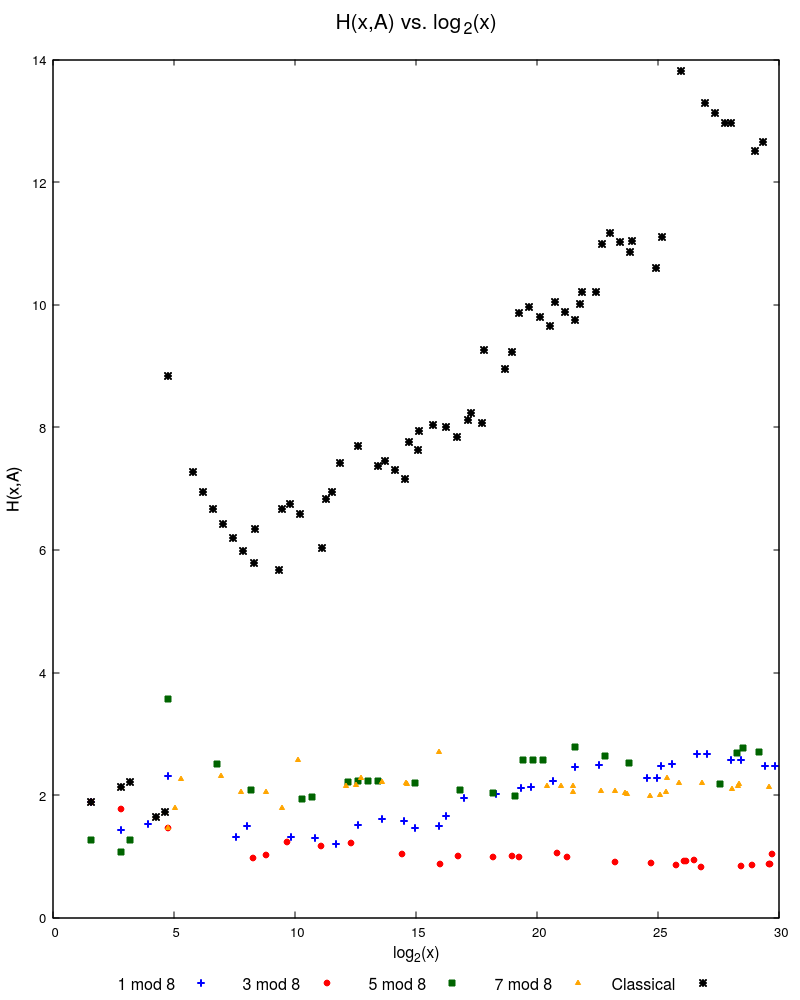
\includegraphics[scale=0.75]{ModAvoidanceAnalysisPics/H_vs_log.png}
    \caption{This graph visualizes how the $H$ values for $1 \Mod{8}$, $5 \Mod{8}$, and $7 \Mod{8}$ compare to each other, and to classical hardness. The log of the record holding numbers, or number of bits needed, is the x-axis, and the hardness measure $H$ as defined in subsection~\ref{subsec:algdefinemeasure} is the y-axis.}
    \label{fig:hvslog}
\end{figure}
Comparing the three unknown mods (1,5, and $7 \Mod{8}$) to the known mod ($3 \Mod{8}$), the known mod case is easier. The known mod case actually slight decreases in hardness as the number of bits increases, meaning that there are fewer odd numbers per bit than the unknown cases. \par
Comparing the unknown cases to themselves, there is no consistent leader among the three as the number of bits increases. However, they all seem to be around within a hardness range of 1-3, with only a couple of exceptions. $7 \Mod{8}$ seems to remain in the same range with no definite increase or decrease, whereas 1 and $5 \Mod{8}$ grow slightly from around 12 bits onward. The growth for both 1 and $5 \Mod{8}$ may be because as numbers get larger, there are more opportunities to visit the $6 \rightarrow 7 \rightarrow 6$ cycle, which rapidly adds more odd numbers. More experiments for higher numbers may need to be run in order to determine whether any of these three unknown cases trend the same way as we add more bits into the computation.
\marginnote{I think an appendix with the table results would at least be a good idea. Printing all the  sequences would be overkill.}
Classical Hardness actually tends to grow linearly against the log scale, meaning that as the input number increases, determining if the input number converges to 1 gets logarithimcally harder. This contrasts to all three mod cases, which tend to stay between values of 1.5 and 3 for $H$ for numbers below 1 billion, meaning that figuring out proofs for their need in the base 8 graph should be easier than proving the Collatz Conjecture.
\subsubsection{Percentage of Sequence Function Results and Analysis} \label{subsubsec:algsinpercentage}
 Figure~\ref{fig:pvslog} shows the results of $P(x,A)$ versus the number of bits.\par 
\begin{figure}
    \centering
    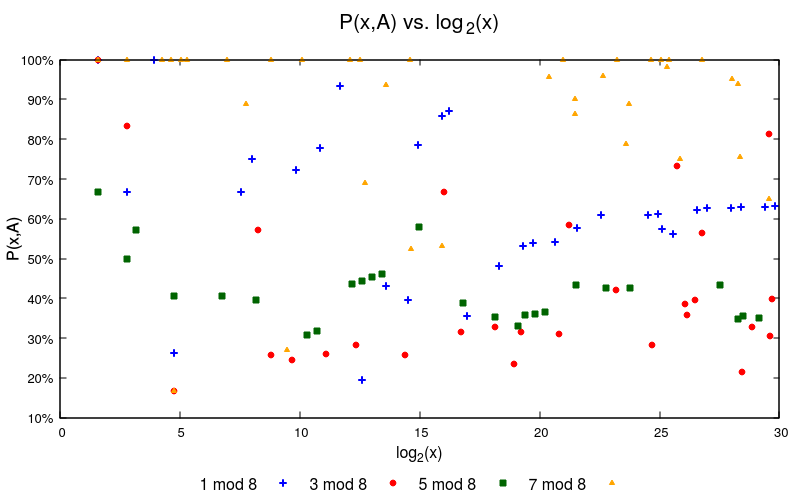
\includegraphics[scale=0.75]{ModAvoidanceAnalysisPics/P_vs_log.png}
    \caption{This graph visualizes how the $P$ values for $1 \Mod{8}$, $5 \Mod{8}$, and $7 \Mod{8}$ compare to each other. The log of the record holding numbers, or number of bits needed, is the x-axis, and the percentage measure $P$ as defined in subsection~\ref{subsec:algdefinemeasure} is the y-axis.}
    \label{fig:pvslog}
\end{figure}

$P(x,A)$, as discussed earlier, is just calculating what percentage of the record sequence contributes to the overall decay of that sequence to 1. \par
Avoiding $7 \Mod{8}$ has the highest percentage overall, with a couple of exceptions. Avoiding $7 \Mod{8}$ causes the sequence to decline rapidly, since the $6 \rightarrow 7 \rightarrow 6$ cycle causes an input number to grow faster than any other cycle in the base 8 graph. Almost all of the records avoiding $7 \Mod{8}$ terminate at 1 instead of actually reaching a number that is $7 \Mod{8}$. \par
Likewise, avoiding $5 \Mod{8}$ tends to have a low percentage overall, and is the least erratic of all four nodes, meaning the standard deviation is lower. Avoiding $5 \Mod{8}$ avoids the 0 self-cycle, which causes many divisions by 2. Numbers having a long sequence of avoiding $5 \Mod{8}$ tend to have a very large number when they hit $5 \Mod{8}$, meaning that often, many more steps in the $3x+1$ mapping must be taken before these numbers converge to 1. \par
$1 \Mod{8}$ is interesting, because as the input numbers grow larger, the line changes from erratic behavior to a more steady percentage between approximately 50\% and 60\% at around 20 bits. This is likely a consequence of the sequence similarity that is seen in larger record sequences that avoid $1 \Mod{8}$, which will be analyzed in subsubsection~\ref{subsubsec:algseqsim}. Further, as mentioned in the cycle analysis for the $4 \rightarrow 6 \rightarrow 3 \rightarrow 2 \rightarrow 5 \rightarrow 0 \rightarrow 4$ cycle (allowing $6 \rightarrow 7 \rightarrow 6$, but avoiding 1), avoiding $1\Mod{8}$ causes a clash between the decay of the 0 self-cycle and the growth of the $6 \rightarrow 7 \rightarrow 6$ cycle, which may explain some of the erratic behavior for $1\Mod{8}$, aside from chain similarity.
$3 \Mod{8}$ tends toward the lowest percentage of all odd numbers, even lower than $5 \Mod{8}$, but also has erratic behavior. This could be explained by the fact that avoiding $3 \Mod{8}$ causes the sequence to follow some combination of the $6 \rightarrow 7 \rightarrow 6$ cycle, the $4 \rightarrow 2 \rightarrow 1 \rightarrow 4$ cycle, or the $4 \rightarrow 2 \rightarrow 5 \rightarrow 0 \rightarrow 4$ cycle with some number of $0$ self-cycles. The first cycle causes growth, whereas all three other cycles cause decay. If the growth cycle is followed, the percentage tends to be lower as the number gets larger, whereas the decay cycles cause the number to shrink, tending the percentages to be higher. This may explain why avoiding $3 \Mod{8}$ causes widely different percentages.
\subsubsection{Sequence similarity analysis} \label{subsubsec:algseqsim}
We analyzed the sequences of the records for 1, 5, and 7 $\Mod{8}$ as well to see if we could find any similarities:
\begin{itemize}
    \item $1\Mod{8}$: There are two groups of records that were particularly interesting: Those from 325,791 to 32,505,681 (call this group $S$), and those from 35,651,835 to 949,643,331 (call this group $T$). Group $S$ numbers all terminated at number 161, and group $T$ numbers all terminated at number 35,369. These sequences all matched \textbf{number-by-number} at least one other sequence starting at most 8
    steps from the beginning. This is a striking similarity meaning that records avoiding $1 \Mod{8}$ might be predictably related to groups $S$ or $T$, or perhaps to other groups.
    \item $7 \Mod{8}$: All record sequences, except for input number 27, terminated at 1. While there was some similarity between sequences (all numbers $\geq 62079$ had the same last 41 numbers), there were many different paths taken from the input, so not as many patterns here.
    \item $5 \Mod{8}$: This had few matches and was the most changing of the records, so it was difficult to pin down any pattern.
\end{itemize}
\section{Paired Base Avoidance Analysis} \label{subsec:algpairedbase}
Because it appears to be difficult to figure out why there is a need for the bases 1, 5, and 7 individually, we have also analyzed pairs of them. Hence, we are trying to find termination of Algorithm~\ref{alg:ColSP} for $|A| = 2$ sets. This section will analyze what happens to $H(x,A)$ and $P(x,A)$ where $A$ is equal to three different base sets: $\{1,5\}$, $\{1,7\}$, and $\{5,7\}$. We already have a straightforward proof for when $A = \{1, 5\}$: Given Lemma~\ref{lem:oneConsumption}, the $6 \rightarrow 7 \rightarrow 6$ cycle can't go on forever, meaning the sequence must eventually follow to $3 \rightarrow 2$, then either 1 or 5. We still included that result to compare it to the other two types of hardness we do not have proofs for: when $A = \{1,7\}$ and $A = \{5,7\}$.

\subsection{Hardness Function Results and Analysis} \label{subsubsec:algmulhardness}
Figure~\ref{fig:h_multivslog} shows the results of $H(x,A)$ versus $\log_2{x}$. Total steps for each mod number were also added in as well.\par
\begin{figure}

    \centering
    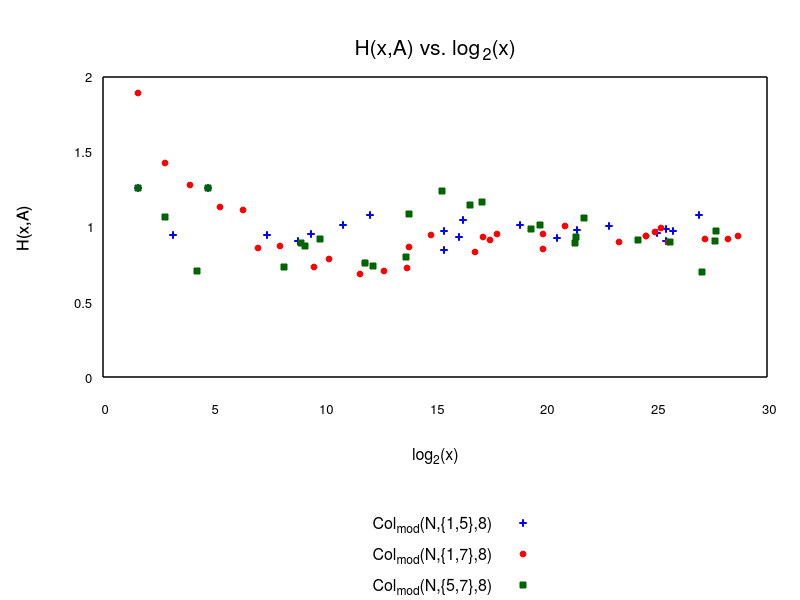
\includegraphics[scale=0.75]{ModAvoidanceAnalysisPics/H_vs_log_multi_base.png}
    \caption{This graph visualizes the $H$ measure for three pairs of avoidance bases for when $A = \{1,5\}$, $A= \{1,7\}$, and $A = \{5,7\}$. The log of the record holding numbers, or number of bits needed, is the x-axis, and the hardness measure $H$ as defined in subsection~\ref{subsec:algdefinemeasure} is the y-axis. Classical Hardness was omitted from this graph to eliminate distortion.}
    \label{fig:h_multivslog}
\end{figure}
These results shocked us. At first thought, it would have appeared that $A = \{1, 5\}$ should be the easiest to determine, because we already had a proof for it. But both $A = \{1, 7\}$ and $A = \{5, 7\}$  had alike predictive hardness to $A = \{1, 5\}$! These numbers suggest that a proof for determining why numbers cannot avoid both $A = \{1, 7\}$, as well as $A = \{5, 7\}$, either should be closer than we anticipated, or our hardness measures are not very good. However, given the fact that $3\Mod{8}$ for the single base cases is clearly easier than 1, 5, or 7 $\Mod{8}$, we have reason to believe this measure should be good. Further investigation needs to be considered.


\subsection{Percentage of Sequence Function Results and Analysis} \label{subsubsec:algmulpercentage}
Figure~\ref{fig:p_multi_vslog} shows the results of $P(x,A)$ versus $\log_2{x}$.\par
\begin{figure}
    \centering
    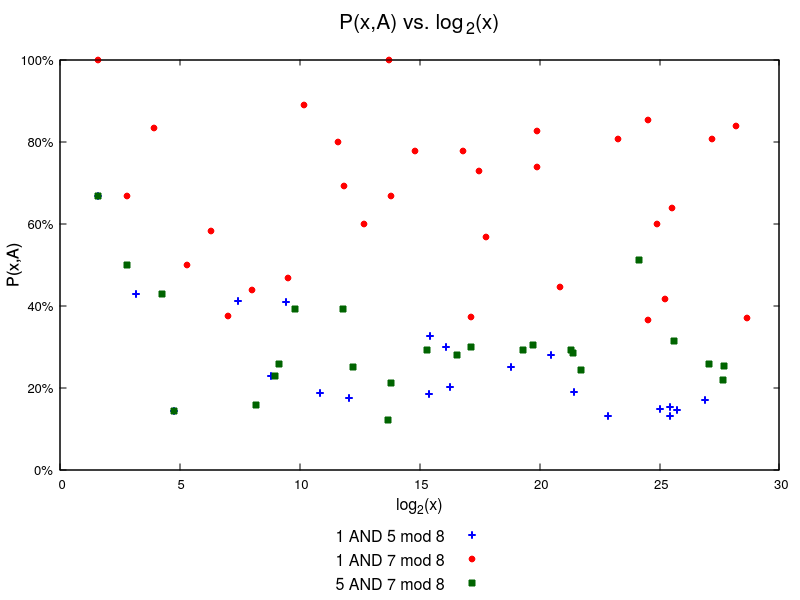
\includegraphics[scale=0.75]{ModAvoidanceAnalysisPics/P_vs_log_multi_base.png}
    \caption{This graph visualizes the $P$ measure for three pairs of avoidance bases for when $A = \{1,5\}$, $A= \{1,7\}$, and $A = \{5,7\}$. The log of the record holding numbers, or number of bits needed, is the x-axis, and the hardness measure $P$ as defined in subsection~\ref{subsec:algdefinemeasure} is the y-axis.}
    \label{fig:p_multi_vslog}
\end{figure}
The avoidance pair $A= \{1,7\}$ makes up the highest percentage of the sequence compared to the other two cases, because avoiding both the $6 \rightarrow 7 \rightarrow 6$ and the $4 \rightarrow 6 \rightarrow 3 \rightarrow 2 \rightarrow 1$ cycles only allows for the sequence to go to $5\Mod{8}$, which causes it to hit the 0 cycle, causing fast decay, like in the $7\Mod{8}$ case. \par
Both of the avoidance pairs $A= \{1,5\}$ and $A= \{5,7\}$ are much closer to each other in percentage of total sequence, although as the numbers grow past 17 bits in size, $A= \{5,7\}$ comprises of the higher percentage of the sequence. A possible explanation is the fact that the $6 \rightarrow 7 \rightarrow 6$ cycle allowed in $A = \{1,5\}$ allows causes a number to grow larger than the $4 \rightarrow 6 \rightarrow 3 \rightarrow 2 \rightarrow 1$ cycle that $A= \{5,7\}$ allows does, and since $A = \{1,5\}$ allows for larger numbers, and the fact that larger numbers generally (but not always) take more steps to decline, that allowing for more growth should mean that the long avoidance sequence for $A = \{1,5\}$ should make up a lower percentage of all odd numbers.
